\documentclass[11pt,a4paper]{article}
\usepackage[utf8]{inputenc}
\usepackage[T1]{fontenc}
\usepackage{amsmath,amssymb,amsfonts,amsthm}
\usepackage{graphicx}
\usepackage{subcaption}
\usepackage{booktabs}
\usepackage{tabularx}
\usepackage{geometry}
\usepackage{hyperref}
\usepackage{xcolor}

\geometry{top=2.2cm,bottom=2.2cm,left=2.2cm,right=2.2cm}
\graphicspath{{plots/frozen_scaling/}{plots/}}

\hypersetup{
    colorlinks=true,
    linkcolor=blue!70!black,
    citecolor=blue!70!black,
    urlcolor=blue!70!black
}

\title{\textbf{Technical Report: Empirical Evaluation of Initial-Condition Scaling and Plateau-Based Neighborhood Selection in Local PCA for Müller--Israel--Stewart Hydrodynamics}}
\author{\textbf{Antigravity QGP Pair Programming}}
\date{\today}

\begin{document}
\maketitle

\begin{abstract}
This report provides a formal mathematical specification and numerical execution report for estimating the local intrinsic dimension of non-equilibrium solutions in Conformal Müller--Israel--Stewart (MIS) hydrodynamics under boost-invariant Bjorken expansion. We implement and evaluate four data normalization procedures: (1) Variant~1, in which scale factors for temperature and pressure anisotropy are frozen from the initial condition standard deviations at $t_0$; (2) Variant~2, in which transverse anisotropy scaling remains frozen at $t_0$ while longitudinal temperature scaling accounts for Bjorken expansion cooling; (3) Variant~3, formulated using the logarithm of temperature with frozen initial scales; and (4) a reference benchmark employing standard slice-by-slice $Z$-score standardization. In each case, local neighborhoods are identified via $k$-nearest neighbors in the scaled metric, empirical covariance matrices are computed, and spectral properties are evaluated using the continuous Participation Ratio ($d_{\mathrm{PR}}$). In addition, we execute a finite-difference plateau-detection algorithm to locate the inflection point $k^*$ where statistical undersampling stabilizes prior to the onset of curvature contamination. All mathematical equations, numerical configurations, phase-space distributions, eigenvalue trajectories, and dimension curves are presented as executed.
\end{abstract}

\vspace{0.5em}
\tableofcontents
\newpage

% ==============================================================================
\section{Hydrodynamic Setup and Initial Phase-Space Configuration}
\label{sec:setup}
% ==============================================================================
We consider a system of boost-invariant, 1D longitudinally expanding quark-gluon plasma described by the conformal Müller--Israel--Stewart (MIS) hydrodynamic equations. The state of the fluid at proper time $\tau$ is specified by the two-dimensional physical state vector:
\begin{equation}
    \mathbf{x}(\tau) = \begin{pmatrix} T(\tau) \\ \mathcal{A}(\tau) \end{pmatrix},
    \label{eq:state_vector}
\end{equation}
where $T(\tau)$ denotes the local temperature (expressed in $\mathrm{fm}^{-1}$, with $1\,\mathrm{fm}^{-1} \approx 197.3\,\mathrm{MeV}$), and $\mathcal{A}(\tau) \equiv (\mathcal{P}_T - \mathcal{P}_L)/\mathcal{P}$ represents the dimensionless pressure anisotropy.

\subsection{Equations of Motion}
From the conservation of energy-momentum $\partial_\mu T^{\mu\nu} = 0$, the temperature evolves according to the exact Bjorken cooling relation:
\begin{equation}
    \tau \frac{dT}{d\tau} = T \left( -\frac{1}{3} + \frac{\mathcal{A}}{18} \right).
    \label{eq:bjorken_cooling}
\end{equation}
For conformal fluids, the pressure anisotropy relaxes toward the universal hydrodynamic attractor $\mathcal{A}_{\mathrm{attr}}(w)$ via:
\begin{equation}
    \tau \frac{d\mathcal{A}}{d\tau} = \frac{1}{C_{\tau_\pi}} \left[ 8 C_\eta - w \mathcal{A} - \frac{2}{9} C_{\tau_\pi} \mathcal{A}^2 \right],
    \label{eq:anisotropy_eq}
\end{equation}
where $C_\eta \equiv \eta/s$, $C_{\tau_\pi} \equiv \tau_\pi T$, and $w \equiv \tau T$ is the dimensionless scaling variable. Linearization around the attractor yields the transverse relaxation rate:
\begin{equation}
    \tau \frac{d\mathcal{A}}{d\tau} \approx -\gamma(w) \big(\mathcal{A} - \mathcal{A}_{\mathrm{attr}}(w)\big), \qquad \gamma(w) \equiv \frac{w}{C_{\tau_\pi}} = \frac{\tau}{\tau_\pi(T)} \gg 1.
    \label{eq:gamma_damping}
\end{equation}

\subsection{Numerical Dataset and Initial Reference Scales}
The dataset analyzed consists of $N = 10\,000$ independent trajectories integrated from initial proper time $\tau_0 = 0.20\,\mathrm{fm}/c$ up to $\tau_{\max} = 3.00\,\mathrm{fm}/c$ sampled across 281 proper-time slices. The initial conditions at $\tau_0$ are distributed across:
\begin{equation}
    T_i(\tau_0) \in [1.0136, \, 6.0811]\,\mathrm{fm}^{-1}, \qquad \mathcal{A}_i(\tau_0) \in [0.0003, \, 5.9996].
\end{equation}
At the initial reference slice $\tau_0 = 0.20\,\mathrm{fm}/c$, the sample statistics evaluated across the ensemble are:
\begin{align}
    \langle T_0 \rangle &= \frac{1}{N} \sum_{i=1}^N T_i(\tau_0) = 3.5528\,\mathrm{fm}^{-1}, \\
    x_T(t_0) &\equiv \sigma_T(\tau_0) = \sqrt{\frac{1}{N-1}\sum_{i=1}^N \big(T_i(\tau_0) - \langle T_0 \rangle\big)^2} = 1.4513\,\mathrm{fm}^{-1}, \\
    x_A(t_0) &\equiv \sigma_{\mathcal{A}}(\tau_0) = \sqrt{\frac{1}{N-1}\sum_{i=1}^N \big(\mathcal{A}_i(\tau_0) - \langle \mathcal{A}_0 \rangle\big)^2} = 1.7219, \\
    x_{\ln T}(t_0) &\equiv \sigma_{\ln T}(\tau_0) = \sqrt{\frac{1}{N-1}\sum_{i=1}^N \left(\ln\frac{T_i(\tau_0)}{\langle T_0 \rangle}\right)^2} = 0.4729.
\end{align}

% ==============================================================================
\section{Coordinate Normalization Schemes}
\label{sec:normalization_schemes}
% ==============================================================================
To evaluate distances between states with different physical units ($T$ in $\mathrm{fm}^{-1}$, $\mathcal{A}$ dimensionless), we define a diagonal scaling transformation $\mathbf{S}^{-1}(t)$.

\subsection{Variant 1: Frozen Scale Normalization}
In Variant~1, the scaling matrix is fixed permanently to the empirical standard deviations measured at $t_0$:
\begin{equation}
    \mathbf{S}_0^{-1} = \begin{pmatrix} 1/x_T(t_0) & 0 \\ 0 & 1/x_A(t_0) \end{pmatrix}.
\end{equation}
The scaled coordinate vector for trajectory $i$ at time $t \ge t_0$ is defined by:
\begin{equation}
    \tilde{\mathbf{x}}_i^{(1)}(t) = \begin{pmatrix} \tilde{T}_i(t) \\ \tilde{\mathcal{A}}_i(t) \end{pmatrix} = \begin{pmatrix} T_i(t) / x_T(t_0) \\ \mathcal{A}_i(t) / x_A(t_0) \end{pmatrix}.
    \label{eq:var1_def}
\end{equation}
The squared distance between two states $i$ and $j$ in this metric is:
\begin{equation}
    d_{ij}^2(t) = \left( \frac{T_i(t) - T_j(t)}{x_T(t_0)} \right)^2 + \left( \frac{\mathcal{A}_i(t) - \mathcal{A}_j(t)}{x_A(t_0)} \right)^2.
\end{equation}
At $t = t_0$, the global covariance matrix is by construction the identity matrix:
\begin{equation}
    \tilde{\mathbf{\Sigma}}_{\mathrm{glob}}(t_0) = \begin{pmatrix} 1 & 0 \\ 0 & 1 \end{pmatrix}.
\end{equation}
For $t > t_0$, the transverse thickness contracts as $\delta\mathcal{A}_\perp(t) \sim x_A(t_0) e^{-\int_{t_0}^t \gamma dt'}$. Because the divisor $x_A(t_0)$ is frozen, the transverse variance decreases toward zero:
\begin{equation}
    \lambda_2(t) \approx \left(\frac{\delta\mathcal{A}_\perp(t)}{x_A(t_0)}\right)^2 \xrightarrow{t \gg t_0} 0.
\end{equation}
However, energy conservation in Bjorken expansion implies $T_i(t) \approx T_i(t_0) (t_0/t)^{1/3}$. Therefore, the temperature spread shrinks kinematically as:
\begin{equation}
    T_i(t) - T_j(t) \approx \big(T_i(t_0) - T_j(t_0)\big) \left(\frac{t_0}{t}\right)^{1/3},
\end{equation}
which causes the global variance of the first coordinate in Variant~1 to contract as:
\begin{equation}
    \mathrm{Var}\big(\tilde{T}(t)\big) = \mathrm{Var}\left(\frac{T(t)}{x_T(t_0)}\right) \approx \left(\frac{t_0}{t}\right)^{2/3} \xrightarrow{t \to \infty} 0.
\end{equation}

\subsection{Variant 2: Cooling-Compensated Scale Normalization}
In Variant~2, the temperature divisor is scaled dynamically by the mean ensemble cooling factor, while the transverse divisor $x_A(t_0)$ remains frozen:
\begin{equation}
    x_T(t) \equiv x_T(t_0) \left( \frac{\langle T(t) \rangle}{\langle T(t_0) \rangle} \right), \qquad x_A = x_A(t_0).
\end{equation}
The scaled coordinates are given by:
\begin{equation}
    \tilde{\mathbf{x}}_i^{(2)}(t) = \begin{pmatrix} T_i(t) / x_T(t) \\ \mathcal{A}_i(t) / x_A(t_0) \end{pmatrix}.
    \label{eq:var2_def}
\end{equation}
Under this formulation, the ensemble variance along the longitudinal temperature direction is maintained at $\mathrm{Var}(\tilde{T}(t)) \approx 1$ for all times $t \ge t_0$.

\subsection{Variant 3: Logarithmic Temperature Normalization}
In Variant~3, the temperature coordinate is expressed in logarithmic form with frozen scales:
\begin{equation}
    \tilde{\mathbf{x}}_i^{(3)}(t) = \begin{pmatrix} \tilde{y}_{T, i}(t) \\ \tilde{\mathcal{A}}_i(t) \end{pmatrix} = \begin{pmatrix} \ln\big(T_i(t)/\langle T_0 \rangle\big) / x_{\ln T}(t_0) \\ \mathcal{A}_i(t) / x_A(t_0) \end{pmatrix}.
    \label{eq:var3_def}
\end{equation}
Because $\ln T_i(t) \approx \ln T_i(t_0) - \frac{1}{3}\ln(t/t_0)$, the cooling term $-\frac{1}{3}\ln(t/t_0)$ shifts all trajectory points by an identical scalar translation. Consequently, the variance $\mathrm{Var}(\tilde{y}_T(t)) \approx 1$ is preserved without requiring explicit time-dependent rescaling.

\subsection{Reference Benchmark: Slice-by-Slice \texorpdfstring{$Z$}{Z}-Score Standardization}
As a reference comparison, we evaluate standard per-slice $Z$-score standardization, where the sample mean $\mu(t)$ and sample standard deviation $\sigma(t)$ are recomputed at each time slice independently:
\begin{equation}
    \tilde{\mathbf{x}}_i^{(\mathrm{Z})}(t) = \begin{pmatrix} \big(T_i(t) - \mu_T(t)\big) / \sigma_T(t) \\ \big(\mathcal{A}_i(t) - \mu_{\mathcal{A}}(t)\big) / \sigma_{\mathcal{A}}(t) \end{pmatrix}.
    \label{eq:zscore_def}
\end{equation}
Under this transformation, both coordinate axes are forced to unit variance ($\sigma_{\tilde{T}} = \sigma_{\tilde{\mathcal{A}}} = 1$) at every time slice $t$.

\subsection{Phase-Space Scatter Evolution}
Figure~\ref{fig:phase_space_evolution} displays the empirical distributions of the trajectory cloud in scaled phase space $(\tilde{x}_1, \tilde{x}_2)$ across four proper-time slices: $\tau = 0.20\,\mathrm{fm}/c$, $\tau = 0.45\,\mathrm{fm}/c$, $\tau = 0.85\,\mathrm{fm}/c$, and $\tau = 2.00\,\mathrm{fm}/c$. Each row corresponds to one of the four normalization schemes, and the markers are color-coded by the initial anisotropy $\mathcal{A}_i(\tau_0)$.

\begin{figure}[htbp]
    \centering
    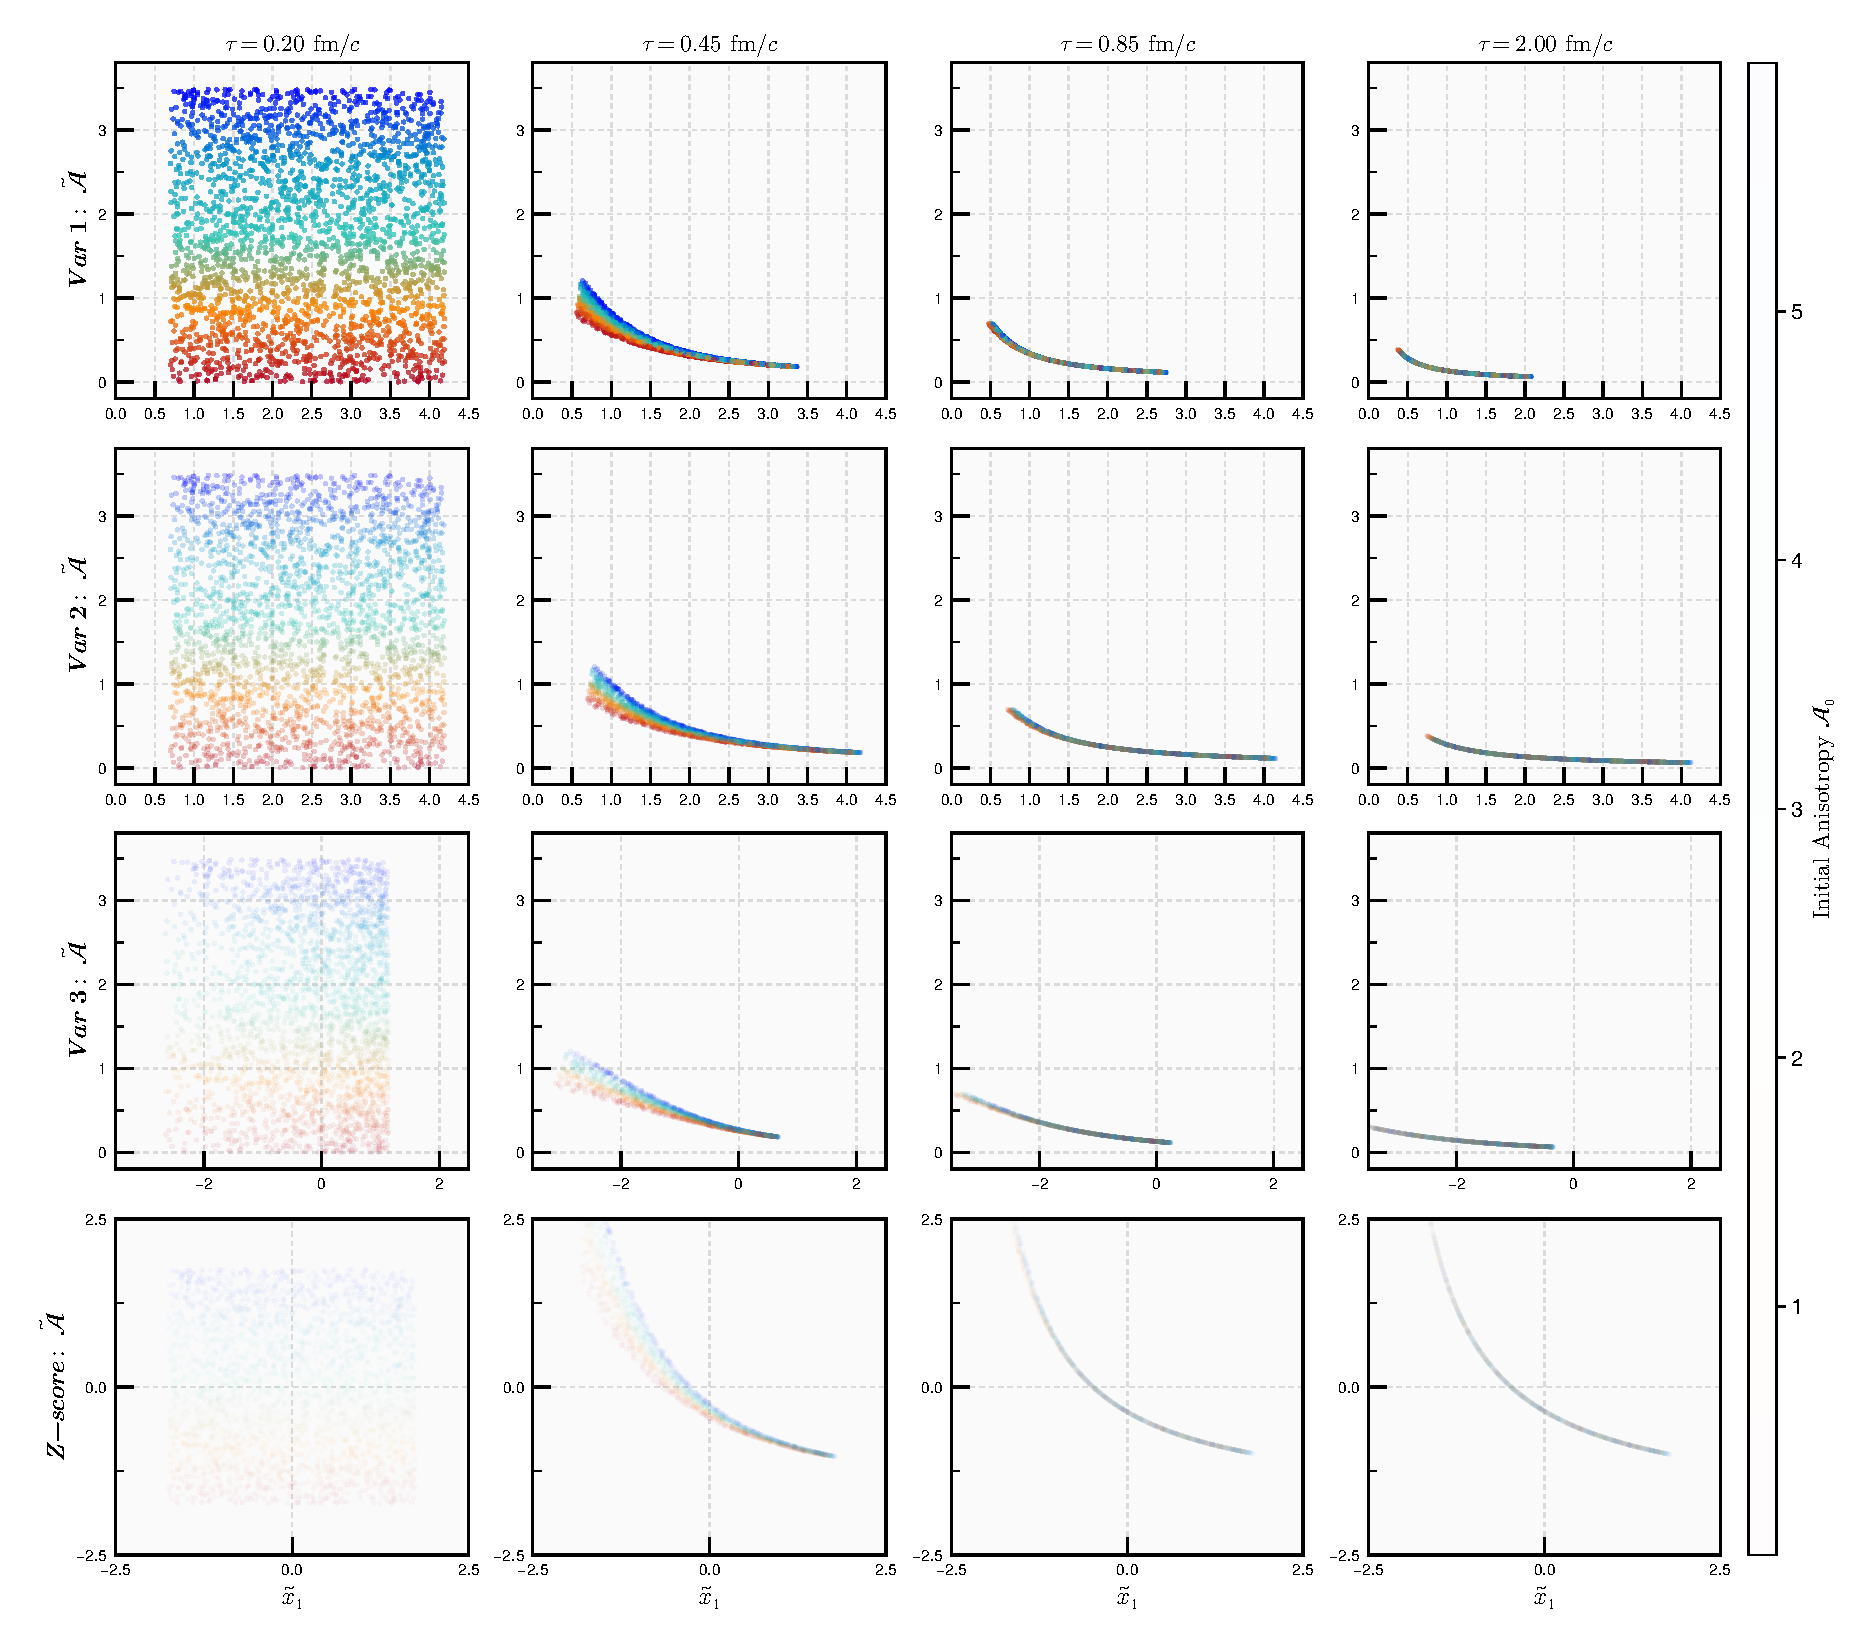
\includegraphics[width=0.98\linewidth]{fig1_phase_space_evolution.pdf}
    \caption{\textbf{Evolution of the trajectory ensemble in scaled phase space.} Slices at proper times $\tau \in \{0.20, 0.45, 0.85, 2.00\}\,\mathrm{fm}/c$ are displayed for Variant~1 (Row~1), Variant~2 (Row~2), Variant~3 (Row~3), and Per-Slice $Z$-Score (Row~4). Points are colored according to initial anisotropy $\mathcal{A}_i(\tau_0) \in [0, 6]$.}
    \label{fig:phase_space_evolution}
\end{figure}

% ==============================================================================
\section{Local PCA and Spectral Eigenvalue Dynamics}
\label{sec:lpca_eigenvalues}
% ==============================================================================
For each trajectory point $\tilde{\mathbf{x}}_i(t)$ in scaled space, we identify its $k$ nearest neighbors $\mathcal{N}_k(\tilde{\mathbf{x}}_i)$ using a $k$-d tree with standard Euclidean metric:
\begin{equation}
    \mathcal{N}_k(\tilde{\mathbf{x}}_i) = \left\{ \tilde{\mathbf{x}}_j \;\middle|\; \|\tilde{\mathbf{x}}_j - \tilde{\mathbf{x}}_i\| \le r_k(\tilde{\mathbf{x}}_i) \right\}, \qquad |\mathcal{N}_k(\tilde{\mathbf{x}}_i)| = k.
\end{equation}
The local sample mean and empirical covariance matrix are:
\begin{equation}
    \bar{\mathbf{x}}_i = \frac{1}{k} \sum_{j \in \mathcal{N}_k(i)} \tilde{\mathbf{x}}_j, \qquad \mathbf{C}_i = \frac{1}{k-1} \sum_{j \in \mathcal{N}_k(i)} (\tilde{\mathbf{x}}_j - \bar{\mathbf{x}}_i)(\tilde{\mathbf{x}}_j - \bar{\mathbf{x}}_i)^T \in \mathbb{R}^{2 \times 2}.
\end{equation}
The eigenvalues $\lambda_1^{(i)} \ge \lambda_2^{(i)} \ge 0$ of $\mathbf{C}_i$ are obtained by spectral decomposition:
\begin{equation}
    \mathbf{C}_i \mathbf{v}_m^{(i)} = \lambda_m^{(i)} \mathbf{v}_m^{(i)}, \qquad m \in \{1, 2\}.
\end{equation}
Here, $\lambda_1$ corresponds to the local sample variance along the principal direction (tangent to the attractor curve at late times), and $\lambda_2$ corresponds to the transverse variance normal to the curve.

\subsection{Continuous Participation Ratio Dimension}
The local Participation Ratio dimension $d_{\mathrm{PR}}(\tilde{\mathbf{x}}_i)$ is evaluated without spectral cutoffs:
\begin{equation}
    d_{\mathrm{PR}}(\tilde{\mathbf{x}}_i) = \frac{\left(\mathrm{Tr}\,\mathbf{C}_i\right)^2}{\mathrm{Tr}\left(\mathbf{C}_i^2\right)} = \frac{\left(\lambda_1^{(i)} + \lambda_2^{(i)}\right)^2}{\left(\lambda_1^{(i)}\right)^2 + \left(\lambda_2^{(i)}\right)^2} = 1 + \frac{2\lambda_1^{(i)}\lambda_2^{(i)}}{\left(\lambda_1^{(i)}\right)^2 + \left(\lambda_2^{(i)}\right)^2}.
    \label{eq:dpr_def}
\end{equation}
The ensemble mean dimension and spectral ratio are:
\begin{equation}
    \langle d_{\mathrm{PR}} \rangle = \frac{1}{N}\sum_{i=1}^N d_{\mathrm{PR}}(\tilde{\mathbf{x}}_i), \qquad \langle \lambda_2 / \lambda_1 \rangle = \frac{1}{N}\sum_{i=1}^N \frac{\lambda_2^{(i)}}{\lambda_1^{(i)}}.
\end{equation}

\subsection{Eigenvalue Trajectories Across Proper Time}
Figure~\ref{fig:eigenvalues_vs_tau} presents the trajectories of the ensemble-averaged eigenvalues $\langle \lambda_1 \rangle$, $\langle \lambda_2 \rangle$, and the spectral ratio $\langle \lambda_2 / \lambda_1 \rangle$ as a function of proper time $\tau \in [0.20, 3.00]\,\mathrm{fm}/c$ evaluated at fixed $k = 16$.
\begin{itemize}
    \item \textbf{Panel (a):} In Variant~1, $\langle \lambda_1 \rangle$ decreases from $1.88 \times 10^{-3}$ at $\tau = 0.20\,\mathrm{fm}/c$ to $5.51 \times 10^{-7}$ at $\tau = 3.00\,\mathrm{fm}/c$, matching the theoretical Bjorken cooling curve $\propto (\tau_0/\tau)^{2/3}$. In Variant~2 and Variant~3, $\langle \lambda_1 \rangle$ stabilizes at asymptotic values of $2.65 \times 10^{-6}$ and $4.21 \times 10^{-6}$. In the per-slice $Z$-score benchmark, $\langle \lambda_1 \rangle$ remains at $\approx 1.89 \times 10^{-5}$.
    \item \textbf{Panel (b):} In all frozen-scale methods (Variants 1, 2, and 3), the transverse eigenvalue $\langle \lambda_2 \rangle$ decays from $1.03 \times 10^{-3}$ at $\tau = 0.20\,\mathrm{fm}/c$ to $7.13 \times 10^{-12}$ at $\tau = 3.00\,\mathrm{fm}/c$. In the per-slice $Z$-score benchmark, $\langle \lambda_2 \rangle$ reaches $1.22 \times 10^{-10}$.
    \item \textbf{Panel (c):} The spectral ratio $\langle \lambda_2 / \lambda_1 \rangle$ decays from $\approx 0.57$ at $\tau_0$ to $7.99 \times 10^{-6}$ (Var~1), $2.85 \times 10^{-6}$ (Var~2), $5.51 \times 10^{-7}$ (Var~3), and $1.31 \times 10^{-6}$ ($Z$-score) at $\tau = 3.00\,\mathrm{fm}/c$.
\end{itemize}

\begin{figure}[htbp]
    \centering
    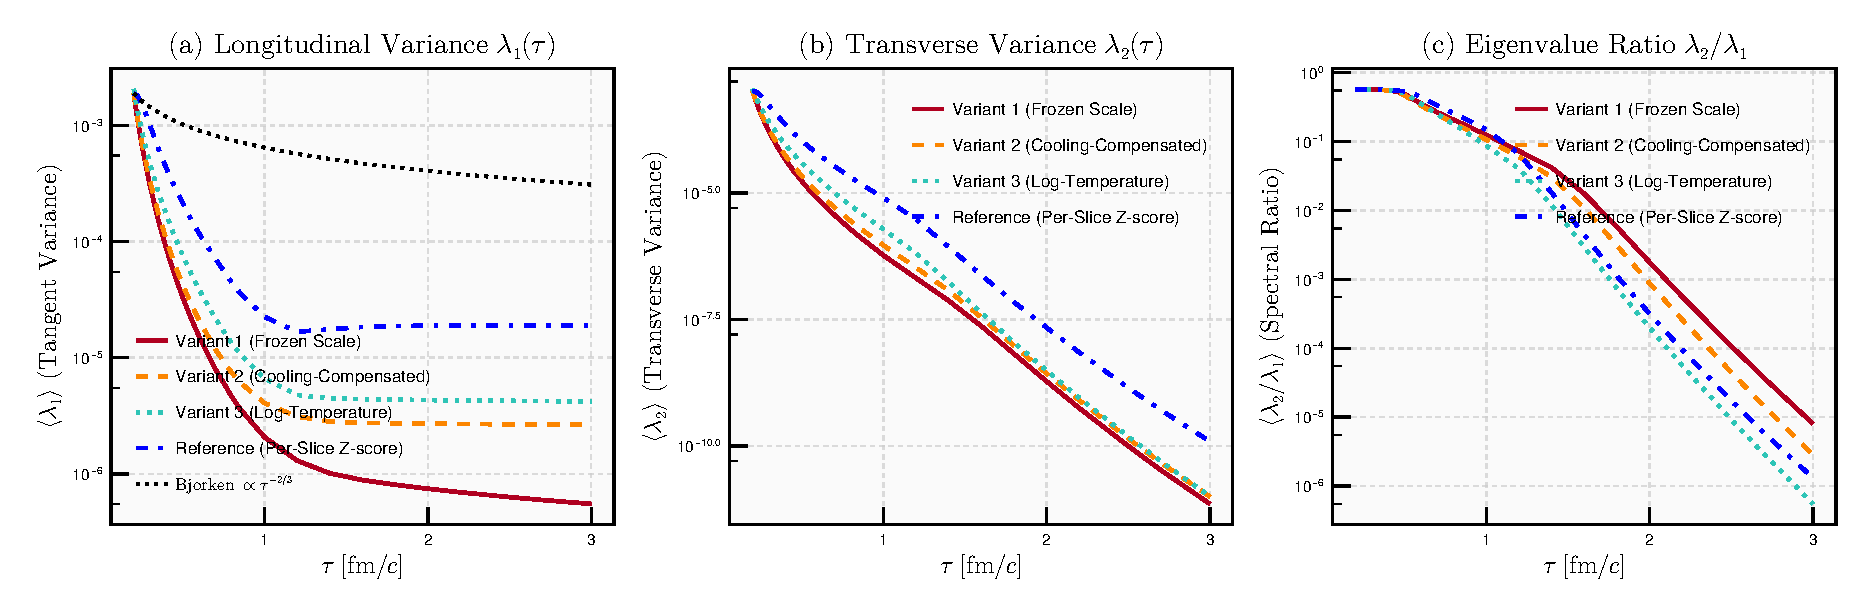
\includegraphics[width=\linewidth]{fig2_eigenvalues_and_ratio_vs_tau.pdf}
    \caption{\textbf{Local PCA eigenvalue dynamics across proper time $\tau$ ($k = 16$).} (a) Mean principal eigenvalue $\langle \lambda_1 \rangle$ with the analytical Bjorken scaling $(\tau_0/\tau)^{2/3}$ indicated by the dotted curve. (b) Mean transverse eigenvalue $\langle \lambda_2 \rangle$. (c) Spectral ratio $\langle \lambda_2 / \lambda_1 \rangle$ on logarithmic scale.}
    \label{fig:eigenvalues_vs_tau}
\end{figure}

% ==============================================================================
\section{Neighborhood Size \texorpdfstring{$k$}{k}-Sweep and Plateau Selection}
\label{sec:k_sweep_plateau}
% ==============================================================================
When estimating local dimension on an ensemble collapsing onto a curved one-dimensional attractor, the dependence of $\langle d_{\mathrm{PR}}(k) \rangle$ on the neighborhood size $k$ reflects a balance between two distinct error sources:
\begin{equation}
    \langle d_{\mathrm{PR}}(k) \rangle \approx d_{\mathrm{true}} - \frac{C_{\mathrm{stat}}}{k} + C_{\mathrm{curv}} \, \kappa^2 \left( \frac{k}{N} \right)^2.
    \label{eq:k_tradeoff}
\end{equation}
\begin{enumerate}
    \item \textbf{Undersampling / Finite-sample bias (small $k$):} For $k < 6$, random configurations of nearest neighbors in 2D space systematically underestimate the lower eigenvalue $\lambda_2$, depressing $d_{\mathrm{PR}}$ toward 1.
    \item \textbf{Plateau interval ($k_{\min} \le k \le k_{\mathrm{curv}}$):} Over intermediate neighborhood sizes, the finite-sample bias decays while the neighborhood diameter remains smaller than the local radius of curvature $R = 1/\kappa$. In this region, $\langle d_{\mathrm{PR}}(k) \rangle$ exhibits a plateau.
    \item \textbf{Curvature contamination (large $k$):} For large $k$, the neighborhood spans an extended arc of the curved attractor curve $\mathcal{A}_{\mathrm{attr}}(w)$. The extrinsic sagitta introduces an apparent normal variance $\lambda_2^{\mathrm{curv}} \propto \kappa^2 (k/N)^4$, which inflates $\langle d_{\mathrm{PR}}(k) \rangle$.
\end{enumerate}

\subsection{Inflection Point Plateau Detection Algorithm}
To locate the center of the plateau automatically without manual parameter tuning, we compute the finite step difference:
\begin{equation}
    \Delta(k) \equiv \Big| \langle d_{\mathrm{PR}}(k+1) \rangle - \langle d_{\mathrm{PR}}(k) \rangle \Big|, \qquad k \in [k_{\min}, \, k_{\max}-1],
    \label{eq:delta_k_def}
\end{equation}
with $k_{\min} = 7$. The optimal plateau neighborhood $k^*$ is identified as the local minimum of $\Delta(k)$:
\begin{equation}
    k^* = \arg\min_{k \ge k_{\min}} \Delta(k).
    \label{eq:k_star_def}
\end{equation}

\subsection{Empirical \texorpdfstring{$k$}{k}-Sweep Results}
Figure~\ref{fig:k_plateau_analysis} displays the sweep of $\langle d_{\mathrm{PR}}(k) \rangle$ (top panels) and the step difference $\Delta(k)$ (bottom panels) across $k \in [3, 50]$ evaluated at three representative proper times: $\tau = 0.20\,\mathrm{fm}/c$, $\tau = 0.55\,\mathrm{fm}/c$, and $\tau = 2.00\,\mathrm{fm}/c$. The detected plateau points $k^*$ are indicated by diamonds and vertical reference lines.
\begin{itemize}
    \item At $\tau = 0.20\,\mathrm{fm}/c$, the cloud is space-filling (2D), and $\langle d_{\mathrm{PR}}(k) \rangle$ increases monotonically toward $\approx 1.92$. The plateau minimum occurs at $k^* = 48$ with $\Delta(k^*) = 5.42 \times 10^{-4}$ and $d_{\mathrm{PR}} = 1.9165$.
    \item At $\tau = 0.55\,\mathrm{fm}/c$, the system is in the hydrodynamizing regime. A clear inflection plateau appears:
    \begin{itemize}
        \item Variant~1: $k^* = 14$, $d_{\mathrm{PR}}(k^*) = 1.6255$, $\Delta(k^*) = 1.74 \times 10^{-4}$.
        \item Variant~2: $k^* = 12$, $d_{\mathrm{PR}}(k^*) = 1.5986$, $\Delta(k^*) = 1.08 \times 10^{-3}$.
        \item Variant~3: $k^* = 16$, $d_{\mathrm{PR}}(k^*) = 1.6427$, $\Delta(k^*) = 1.72 \times 10^{-3}$.
        \item Per-slice $Z$-score: $k^* = 18$, $d_{\mathrm{PR}}(k^*) = 1.7513$, $\Delta(k^*) = 1.85 \times 10^{-4}$.
    \end{itemize}
    \item At $\tau = 2.00\,\mathrm{fm}/c$, the cloud is collapsed onto the 1D attractor. The plateau gives $d_{\mathrm{PR}} = 1.0003$ (Var~1), $1.0002$ (Var~2), $1.0000$ (Var~3), and $1.0001$ ($Z$-score), with step differences $\Delta(k^*) < 1.5 \times 10^{-5}$.
\end{itemize}

\begin{figure}[htbp]
    \centering
    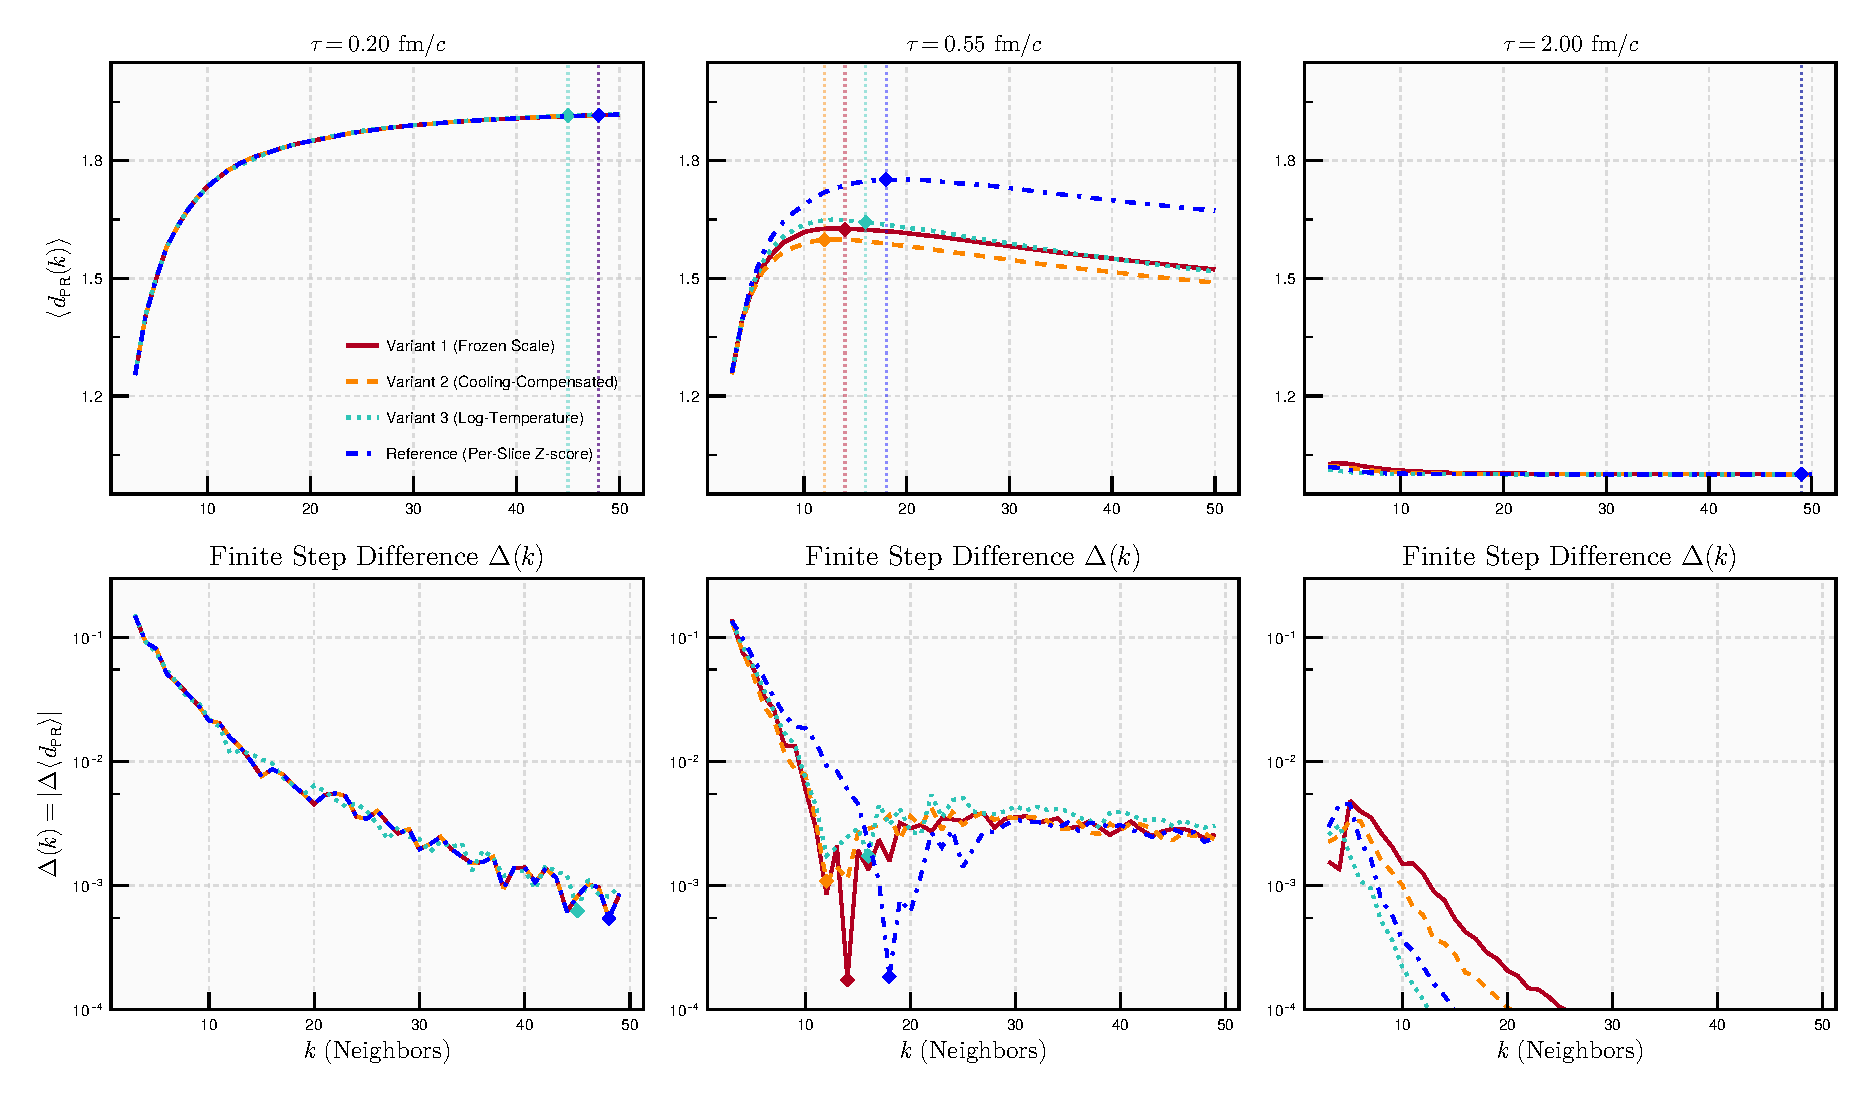
\includegraphics[width=\linewidth]{fig3_k_plateau_analysis.pdf}
    \caption{\textbf{Neighborhood size $k$-sweep and automated plateau detection.} Top panels: $\langle d_{\mathrm{PR}}(k) \rangle$ for $k \in [3, 50]$ at proper times $\tau = 0.20\,\mathrm{fm}/c$, $\tau = 0.55\,\mathrm{fm}/c$, and $\tau = 2.00\,\mathrm{fm}/c$. Bottom panels: Step difference $\Delta(k) = |\langle d_{\mathrm{PR}}(k+1) \rangle - \langle d_{\mathrm{PR}}(k) \rangle|$. Diamond markers denote the detected plateau minima $k^*$.}
    \label{fig:k_plateau_analysis}
\end{figure}

% ==============================================================================
\section{Dimensional Trajectories Across Proper Time}
\label{sec:trajectories}
% ==============================================================================
Figure~\ref{fig:dimension_trajectories} displays the time evolution of the ensemble-averaged Participation Ratio dimension $\langle d_{\mathrm{PR}}(\tau) \rangle$ across proper times $\tau \in [0.20, 3.00]\,\mathrm{fm}/c$.
\begin{itemize}
    \item \textbf{Panel (a) (Fixed Neighborhood $k = 16$):} At early times ($\tau \le 0.35\,\mathrm{fm}/c$), all methods yield $\langle d_{\mathrm{PR}} \rangle \approx 1.82$. During the collapse phase ($\tau \in [0.45, 1.00]\,\mathrm{fm}/c$), Variant~1, Variant~2, and Variant~3 decay rapidly (e.g., reaching $1.59$--$1.64$ at $\tau = 0.55\,\mathrm{fm}/c$), whereas the per-slice $Z$-score benchmark remains higher at $1.7480$. For $\tau \ge 2.00\,\mathrm{fm}/c$, all methods converge asymptotically to $1.00$.
    \item \textbf{Panel (b) (Adaptive Neighborhood $k^*(\tau)$):} Evaluating $d_{\mathrm{PR}}$ at the adaptive plateau value $k^*(\tau)$ determined by Eq.~\eqref{eq:k_star_def} yields $\langle d_{\mathrm{PR}} \rangle \approx 1.90$ at $\tau_0 = 0.20\,\mathrm{fm}/c$, decays through the inflection values at intermediate times, and terminates at $1.0000$ on the attractor.
\end{itemize}

\begin{figure}[htbp]
    \centering
    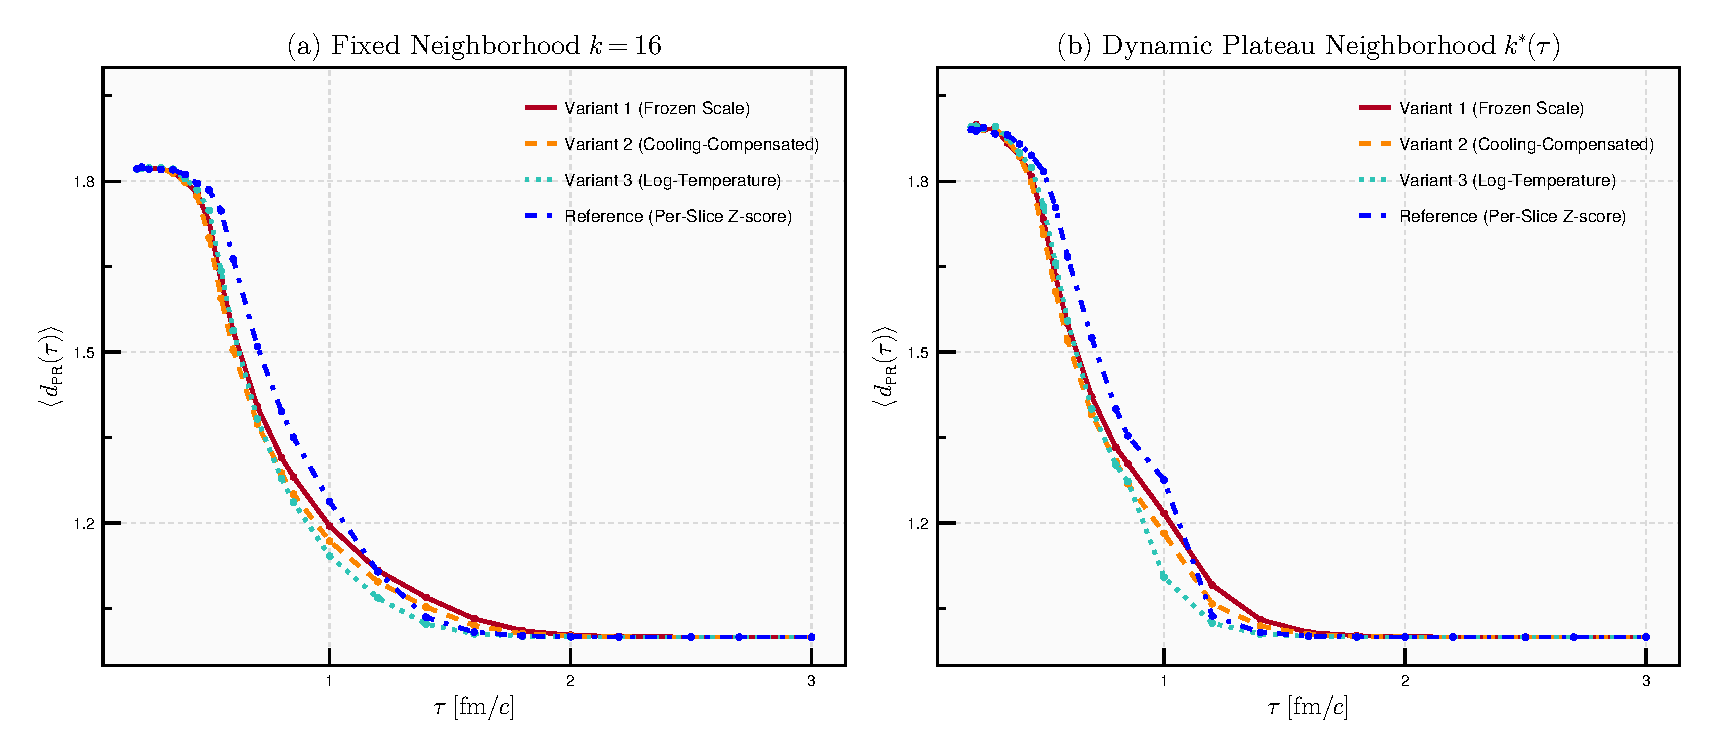
\includegraphics[width=0.92\linewidth]{fig4_dimension_trajectories.pdf}
    \caption{\textbf{Dimensional trajectories $\langle d_{\mathrm{PR}}(\tau) \rangle$ across proper time.} (a) Evaluated at fixed neighborhood size $k = 16$. (b) Evaluated dynamically at the adaptive plateau neighborhood $k^*(\tau)$.}
    \label{fig:dimension_trajectories}
\end{figure}

% ==============================================================================
\section{Tabulated Numerical Summary}
\label{sec:numerical_table}
% ==============================================================================
Table~\ref{tab:numerical_results} compiles the exact numerical values obtained from the simulation runs across representative proper times $\tau$ for all four normalization schemes.

\begin{table}[htbp]
\centering
\small
\caption{\textbf{Numerical summary of local PCA and participation ratio dimension across proper time $\tau$.}}
\label{tab:numerical_results}
\resizebox{\linewidth}{!}{%
\begin{tabular}{llcccccc}
\toprule
$\tau$ [$\mathrm{fm}/c$] & Method & $\langle d_{\mathrm{PR}}(k=16) \rangle$ & $k^*$ & $\langle d_{\mathrm{PR}}(k^*) \rangle$ & $\langle \lambda_1 \rangle$ & $\langle \lambda_2 \rangle$ & $\langle \lambda_2/\lambda_1 \rangle$ \\
\midrule
0.200 & Var 1 (Frozen)      & 1.8217 & 34 & 1.8993 & $1.884 \times 10^{-3}$ & $1.034 \times 10^{-3}$ & 0.5701 \\
      & Var 2 (Compensated) & 1.8217 & 34 & 1.8993 & $1.884 \times 10^{-3}$ & $1.034 \times 10^{-3}$ & 0.5701 \\
      & Var 3 (Log $T$)     & 1.8211 & 31 & 1.8935 & $2.056 \times 10^{-3}$ & $1.124 \times 10^{-3}$ & 0.5699 \\
      & Per-Slice $Z$-score & 1.8217 & 34 & 1.8993 & $1.884 \times 10^{-3}$ & $1.034 \times 10^{-3}$ & 0.5701 \\
\addlinespace
0.350 & Var 1 (Frozen)      & 1.8158 & 32 & 1.8737 & $1.530 \times 10^{-4}$ & $8.317 \times 10^{-5}$ & 0.5642 \\
      & Var 2 (Compensated) & 1.8139 & 32 & 1.8714 & $1.763 \times 10^{-4}$ & $9.570 \times 10^{-5}$ & 0.5628 \\
      & Var 3 (Log $T$)     & 1.8210 & 30 & 1.8762 & $2.701 \times 10^{-4}$ & $1.469 \times 10^{-4}$ & 0.5701 \\
      & Per-Slice $Z$-score & 1.8200 & 34 & 1.8879 & $6.344 \times 10^{-4}$ & $3.431 \times 10^{-4}$ & 0.5696 \\
\addlinespace
0.550 & Var 1 (Frozen)      & 1.6238 & 14 & 1.6255 & $2.198 \times 10^{-5}$ & $1.126 \times 10^{-5}$ & 0.4129 \\
      & Var 2 (Compensated) & 1.5945 & 12 & 1.5986 & $2.924 \times 10^{-5}$ & $1.476 \times 10^{-5}$ & 0.3933 \\
      & Var 3 (Log $T$)     & 1.6427 & 16 & 1.6427 & $5.341 \times 10^{-5}$ & $2.740 \times 10^{-5}$ & 0.4227 \\
      & Per-Slice $Z$-score & 1.7480 & 18 & 1.7513 & $1.553 \times 10^{-4}$ & $7.881 \times 10^{-5}$ & 0.5021 \\
\addlinespace
0.850 & Var 1 (Frozen)      & 1.2810 & 11 & 1.2924 & $3.635 \times 10^{-6}$ & $1.402 \times 10^{-6}$ & 0.1824 \\
      & Var 2 (Compensated) & 1.2510 &  9 & 1.2663 & $6.141 \times 10^{-6}$ & $2.089 \times 10^{-6}$ & 0.1613 \\
      & Var 3 (Log $T$)     & 1.2369 &  9 & 1.2615 & $1.080 \times 10^{-5}$ & $4.281 \times 10^{-6}$ & 0.1492 \\
      & Per-Slice $Z$-score & 1.3506 & 10 & 1.3613 & $3.626 \times 10^{-5}$ & $1.587 \times 10^{-5}$ & 0.2253 \\
\addlinespace
1.000 & Var 1 (Frozen)      & 1.1949 &  9 & 1.2107 & $2.071 \times 10^{-6}$ & $5.871 \times 10^{-7}$ & 0.1239 \\
      & Var 2 (Compensated) & 1.1684 & 11 & 1.1818 & $4.069 \times 10^{-6}$ & $9.258 \times 10^{-7}$ & 0.1060 \\
      & Var 3 (Log $T$)     & 1.1423 &  9 & 1.1703 & $6.617 \times 10^{-6}$ & $1.926 \times 10^{-6}$ & 0.0867 \\
      & Per-Slice $Z$-score & 1.2379 & 10 & 1.2629 & $2.250 \times 10^{-5}$ & $8.081 \times 10^{-6}$ & 0.1478 \\
\addlinespace
2.000 & Var 1 (Frozen)      & 1.0035 & 34 & 1.0007 & $7.444 \times 10^{-7}$ & $1.886 \times 10^{-9}$ & $1.759 \times 10^{-3}$ \\
      & Var 2 (Compensated) & 1.0017 & 34 & 1.0004 & $2.707 \times 10^{-6}$ & $2.686 \times 10^{-9}$ & $8.702 \times 10^{-4}$ \\
      & Var 3 (Log $T$)     & 1.0004 & 34 & 1.0001 & $4.321 \times 10^{-6}$ & $3.086 \times 10^{-9}$ & $1.972 \times 10^{-4}$ \\
      & Per-Slice $Z$-score & 1.0006 & 34 & 1.0001 & $1.886 \times 10^{-5}$ & $2.180 \times 10^{-8}$ & $3.143 \times 10^{-4}$ \\
\addlinespace
3.000 & Var 1 (Frozen)      & 1.0000 & 34 & 1.0000 & $5.509 \times 10^{-7}$ & $7.125 \times 10^{-12}$ & $8.000 \times 10^{-6}$ \\
      & Var 2 (Compensated) & 1.0000 & 34 & 1.0000 & $2.650 \times 10^{-6}$ & $9.901 \times 10^{-12}$ & $2.848 \times 10^{-6}$ \\
      & Var 3 (Log $T$)     & 1.0000 & 34 & 1.0000 & $4.210 \times 10^{-6}$ & $9.949 \times 10^{-12}$ & $5.511 \times 10^{-7}$ \\
      & Per-Slice $Z$-score & 1.0000 & 31 & 1.0000 & $1.894 \times 10^{-5}$ & $1.221 \times 10^{-10}$ & $1.312 \times 10^{-6}$ \\
\bottomrule
\end{tabular}%
}
\end{table}

\end{document}
